\section{Results}
\label{sec:results}

\subsection{Certified banks}

Every puzzle in the four banks was certified unique by MiniSat and, independently, by CP-SAT, and every clue of every puzzle is necessary. Table~\ref{tab:bank} shows the ladder levels. Minimal puzzles rarely sit at L1: removing every redundant clue removes the easy routes, so the weakest engine that suffices is usually single-constraint elimination (L2) or failed-literal probing (L3). Minimal Sudoku is the exception, because with 9 digits per unit a few givens already create hidden singles; across 9{,}500 random minimal Sudoku none needed more than L3. The ladder separates the families: Killer reaches L4 in a fifth of the puzzles and L5 in four, zebra reaches L4 in about one in nine, and $5{\times}5$ Futoshiki never needs more than L3. Puzzles generated from the hard text templates have a similar level distribution to plain ones, because the templates change the wording, not the constraint.

\begin{table*}[t]
\centering
\caption{Ladder levels of the certified banks (minimal puzzles). All puzzles were certified unique by two solvers.}
\label{tab:bank}
\small
\begin{tabular}{lrrrrrrr}
\toprule
Family & $n$ & L1 & L2 & L3 & L4 & L5 & clues (mean) \\
\midrule
\rows{bank_rows}
\bottomrule
\end{tabular}
\end{table*}

\subsection{E1: how often is a single encoding wrong?}

Figure~\ref{fig:example} shows one puzzle end to end: the text, the two Sonnet encodings (they differ in form on three clues and are proved equivalent), and the chain of forced facts with the minimal clue set behind each. Table~\ref{tab:e1} and Figure~\ref{fig:e1} give the error rates.

On plain template text no encoder made an error: 0 of 3$\times$\EOnePlainClues clue encodings were wrong. On hard templates Sonnet~A produced no wrong puzzle, Sonnet~B \EOneHardErrNB and Haiku \EOneHardErrNC of 100 (\EOneHardErrC). On paraphrased text all three encoders were wrong on 7--8 of \EOneParaN puzzles (Sonnet~A \EOneParaErrA). These rates are low and their intervals are wide; the more useful result is the audit of what went wrong (Section~\ref{sec:audit}).

\begin{table*}[t]
\centering
\caption{E1. Puzzles with a wrong encoding (in brackets: wrong clue encodings) for each encoder, and puzzles on which a pair of encoders disagrees (in brackets: puzzles with at least one wrong encoder in the pair that the dual check flagged / all such puzzles).}
\label{tab:e1}
\small
\setlength{\tabcolsep}{4pt}
\begin{tabular}{lrcccccc}
\toprule
 & & \multicolumn{3}{c}{wrong single encoding} & \multicolumn{3}{c}{dual check: disagree (caught/with error)} \\
\cmidrule(lr){3-5}\cmidrule(lr){6-8}
Text & $n$ & Sonnet A & Sonnet B & Haiku C & A--B & A--C & B--C \\
\midrule
\rows{e1_rows}
\bottomrule
\end{tabular}
\end{table*}

\begin{figure*}[t]
\centering
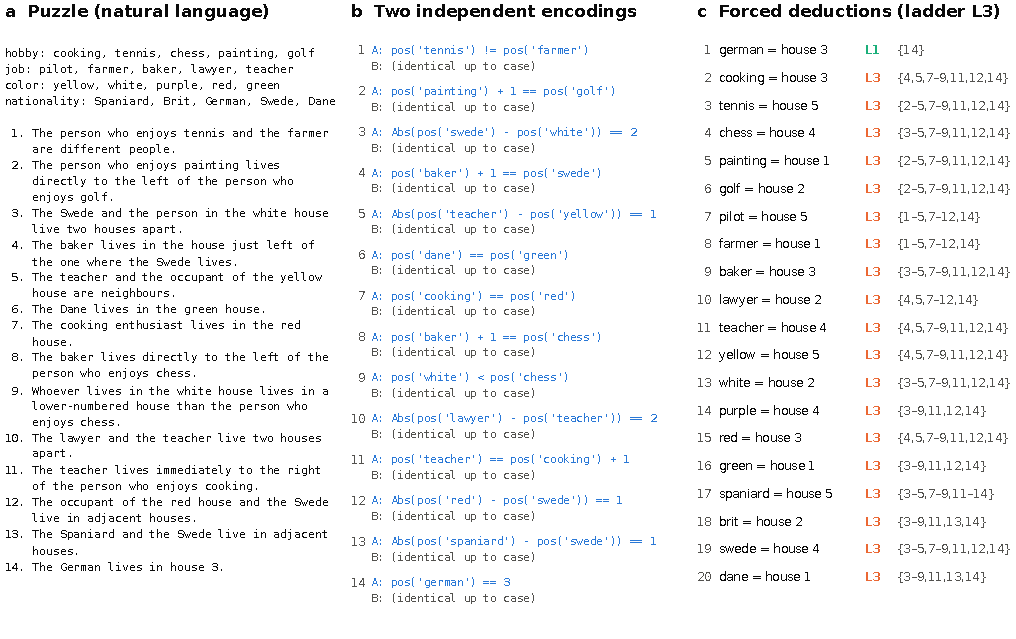
\includegraphics[width=\textwidth]{../figures/fig1_example.pdf}
\caption{One zebra puzzle through the pipeline. (a) The text given to the encoders. (b) The two Sonnet encodings in the position DSL; three clues are written differently and z3 proves $A \oplus B$ unsatisfiable. (c) Every fact of the solution in the order the ladder derives it, the strongest rule needed so far, and a minimal set of clues that forces it. The puzzle is L3: after one unit-propagation step every further fact needs failed-literal probing, and most explanations need 8--13 of the 14 clues.}
\label{fig:example}
\end{figure*}

\begin{figure}[t]
\centering
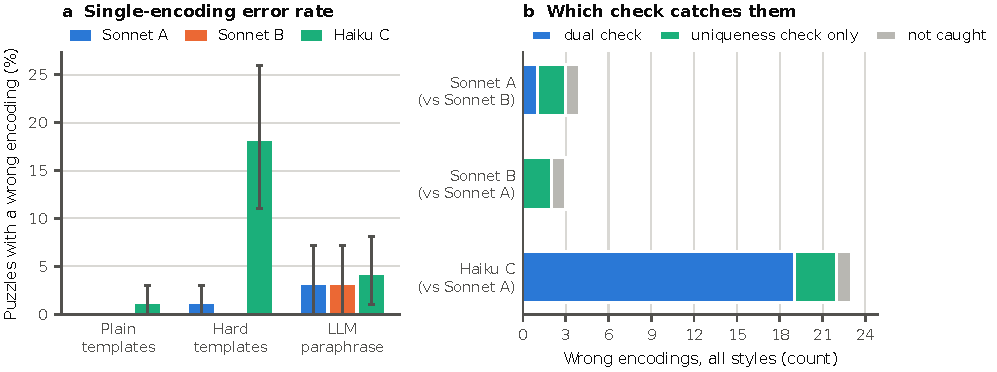
\includegraphics[width=\columnwidth]{../figures/fig2_faithfulness.pdf}
\caption{E1. (a) Share of puzzles with a wrong single encoding, with 95\% bootstrap intervals. (b) For each encoder, how its wrong encodings were detected: by disagreement with its partner encoding, or only because the wrongly encoded puzzle no longer had a unique solution. No wrong encoding escaped both checks.}
\label{fig:e1}
\end{figure}

\paragraph{Detection.} The dual check flagged every puzzle on which exactly one encoder of a pair was wrong. It missed the errors that both encoders shared: on paraphrased text the two Sonnet encodings disagreed on no puzzle at all, although both were wrong on the same 7. Each of those wrong encodings, however, made the encoded puzzle lose its unique solution, so the uniqueness check rejected it. Across all 299 puzzles and all three encoders, no wrong encoding passed both checks (Figure~\ref{fig:e1}b). Uniqueness works as a second detector because a minimal puzzle has no slack: changing the meaning of one clue almost always either removes the intended solution or admits a second one.

\paragraph{Audit.}\label{sec:audit} We read every clue-level error by hand (\texttt{results/e1/audit.md}). There were four groups.
(i) \emph{An ambiguous template of our own} (\EOneTaxTooStrong clue encodings per encoder): ``At least one house separates X and Y'' was generated for ``X and Y are not neighbours'' ($|p_X-p_Y|\neq1$, which allows the same house), and all three encoders read it as $|p_X-p_Y|\ge2$. Their reading is the natural one; the template is wrong. Because the clue is still true of the solution, no answer changed, and neither check can see the error; only the formal ground truth revealed it.
(ii) \emph{Counting from the right}: ``the fourth house from the right'' encoded as house~4 (Haiku 5 clues, Sonnet~B 1).
(iii) \emph{Direction flips}: ``the left-hand neighbour of the German drinks juice'' encoded with the German on the left (2 clues).
(iv) \emph{Paraphrase drift}: Sonnet, asked to keep the meaning exactly, rewrote ``exactly one house between X and Y'' as ``two houses separate X and Y'' in 7 puzzles. The encoders then encoded what the text said. This is an error of the text, not of the encoding, and dual encoding by construction cannot catch it.

\subsection{E2: LLM-written puzzles without and with the loop}

Sonnet's puzzles were almost always valid (Table~\ref{tab:e2}): \ETwoValid of \ETwoN parsed, had a unique solution equal to the stated one, and were fair. One Sudoku had a stated solution different from its true unique solution, and one Futoshiki had several solutions; one round of solver feedback repaired both (\ETwoValidRepair of \ETwoN). The zebra puzzles' two encodings never disagreed.

The puzzles were, however, easy and redundant (Figure~\ref{fig:e2}). All 20 Sudoku had exactly 30 givens and were solved by unit propagation alone; half of the Killer puzzles were L1. On average \ETwoSudokuRed of a Sudoku's givens, \ETwoKillerRed of a Killer puzzle's clues and \ETwoFutoshikiRed of a Futoshiki puzzle's clues could each be removed without losing uniqueness; for zebra puzzles the figure was \ETwoZebraRed. Minimising the LLM puzzles with the solver raised their level (Sudoku: \ETwoSudokuMinLC of 20 reached L3; zebra: \ETwoZebraMinLC of 40). The 20 Sudoku used only \ETwoSudokuMasks distinct layouts of givens; \ETwoSudokuWikiMask used the layout of the example puzzle on the English Wikipedia Sudoku page and \ETwoSudokuWikiSame reproduced that puzzle exactly. LLM-written puzzles are thus valid but not a good source of hard or novel instances, and copying is a real risk for benchmarks built this way.

\begin{table*}[t]
\centering
\caption{E2. Validity, level and redundancy of 100 puzzles written by Sonnet. ``Valid'' = parses, unique, matches the stated solution and fair (L1--L3). Levels are given as L1/L2/L3 counts before and after solver minimisation.}
\label{tab:e2}
\small
\begin{tabular}{lrrrrrccrc}
\toprule
Family & $n$ & unique & as stated & valid & after repair & levels (LLM) & levels (min.) & redundancy & clues \\
\midrule
\rows{e2_rows}
\bottomrule
\end{tabular}
\end{table*}

\begin{figure}[t]
\centering
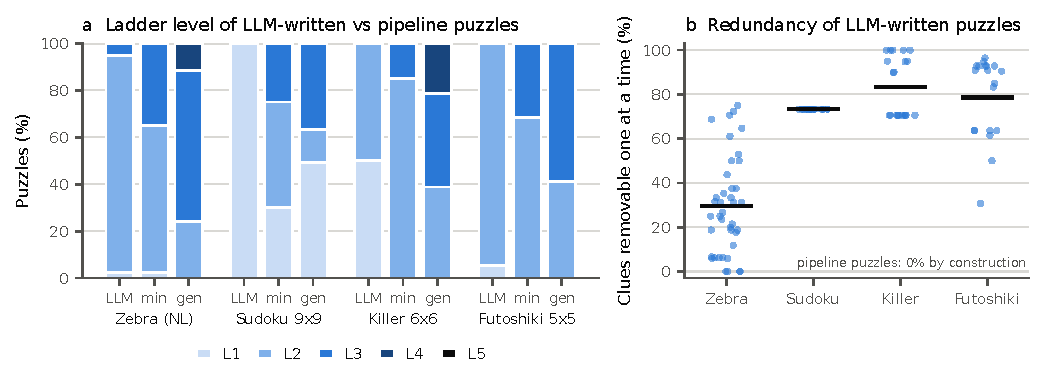
\includegraphics[width=\columnwidth]{../figures/fig3_validity.pdf}
\caption{E2. (a) Ladder levels of the LLM-written puzzles, of the same puzzles after solver minimisation, and of the pipeline's own bank. (b) Fraction of clues that can each be removed without losing uniqueness; the pipeline's puzzles have none by construction.}
\label{fig:e2}
\end{figure}

\subsection{E3: the ladder, solver effort and LLM accuracy}

\paragraph{Ladder versus solver metrics.} Within every family the ladder level tracks solver effort and explanation size (Figure~\ref{fig:metrics}, Table~\ref{tab:rho}). The Spearman correlation of level with MiniSat conflicts was \RhoZebraConflicts (zebra), \RhoSudokuConflicts (Sudoku), \RhoKillerConflicts (Killer) and \RhoFutoshikiConflicts (Futoshiki); with the share of variables fixed by unit propagation it was between \RhoSudokuUpClosure and \RhoZebraUpClosure. The level is not a proxy for the number of clues: in Sudoku the correlation with the number of givens was \RhoSudokuNClues, and in the other families harder puzzles had \emph{fewer} clues. Mean explanation size rises with level, so harder puzzles are also those in which each fact depends on more clues at once.

\begin{figure*}[t]
\centering
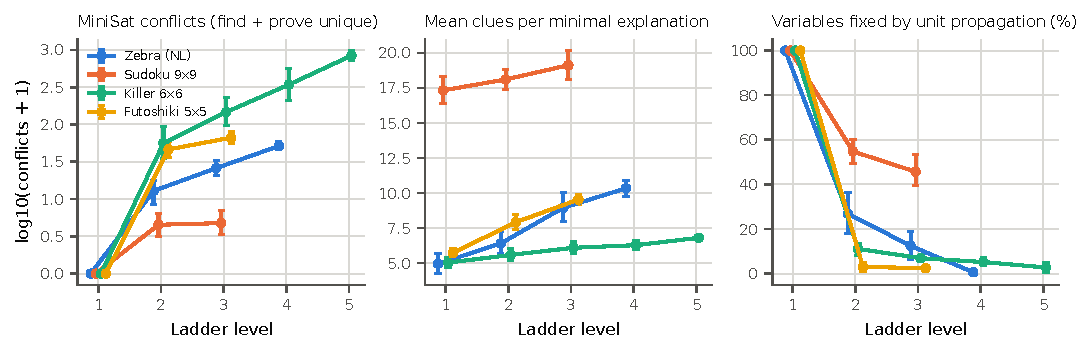
\includegraphics[width=\textwidth]{../figures/fig4_ladder_metrics.pdf}
\caption{E3. Solver-side metrics by ladder level for the 116 selected puzzles (means with 95\% bootstrap intervals). L1 cells of zebra, Killer and Futoshiki contain augmented puzzles.}
\label{fig:metrics}
\end{figure*}

\begin{table*}[t]
\centering
\caption{E3. Spearman correlation of ladder level with solver metrics, with 95\% bootstrap intervals.}
\label{tab:rho}
\small
\setlength{\tabcolsep}{3pt}
\begin{tabular}{lcccc}
\toprule
Metric & Zebra & Sudoku & Killer & Futoshiki \\
\midrule
\rows{e3rho_rows}
\bottomrule
\end{tabular}
\end{table*}

\paragraph{Ladder versus LLM accuracy.} Table~\ref{tab:acc} and Figure~\ref{fig:acc} give the exact-solution rates. Every model solved every zebra puzzle at every level, including the 8 L4 puzzles. Opus solved all \EThreeN puzzles; Sonnet missed one L5 Killer puzzle (with 35 of 36 cells right). Only Haiku made more than isolated errors, and mostly on Sudoku (\EThreeSudokuHaiku\% exact). Haiku's Sudoku accuracy fell from 6 of 8 at L1 and L2 to 3 of 8 at L3, but this drop needs care: \EThreeSudokuHaikuUnans of its 24 Sudoku items were left unanswered, 5 of them L3, and 5 of the 6 came from one call that gave up on its whole batch of five. Among the items Haiku did answer, it solved \EThreeSudokuHaikuAnsLA at L1, \EThreeSudokuHaikuAnsLB at L2 and \EThreeSudokuHaikuAnsLC at L3. Whether giving up is itself a sign of difficulty cannot be separated here from the batch it happened in.

Formally, on the family--model cells that are not at ceiling (Sudoku, Killer and Futoshiki for Haiku and Sonnet; $n=\LogitN$), the logistic slope of exact solution on level was \LogitLevel (95\% cluster-bootstrap interval \LogitLevelLo{} to \LogitLevelHi; $p=\LogitLevelP$). A linear mixed model of cell accuracy over all 348 attempts gave a level slope of \MixedLevel{} per level (SE \MixedLevelSE, $p=\MixedLevelP$). Adding the level to a model with MiniSat conflicts, explanation size and number of clues lowered the AIC from \AICMetrics{} to \AICMetricsLevel{}, so the ladder carries some information that raw solver effort does not, but the evidence is weak. The honest summary is that for current models these puzzle sizes are mostly too easy for the ladder to predict accuracy: it predicts solver effort well and LLM failure poorly, because there are few failures to predict.

\begin{table}[t]
\centering
\caption{E3. Exact solutions (\%) with 95\% bootstrap intervals, all levels pooled. Unanswered items count as wrong (Haiku: 6 Sudoku and 2 Futoshiki items).}
\label{tab:acc}
\small
\setlength{\tabcolsep}{3pt}
\begin{tabular}{lccc}
\toprule
Family & Haiku & Sonnet & Opus \\
\midrule
\rows{e3acc_rows}
\bottomrule
\end{tabular}
\end{table}

\begin{figure*}[t]
\centering
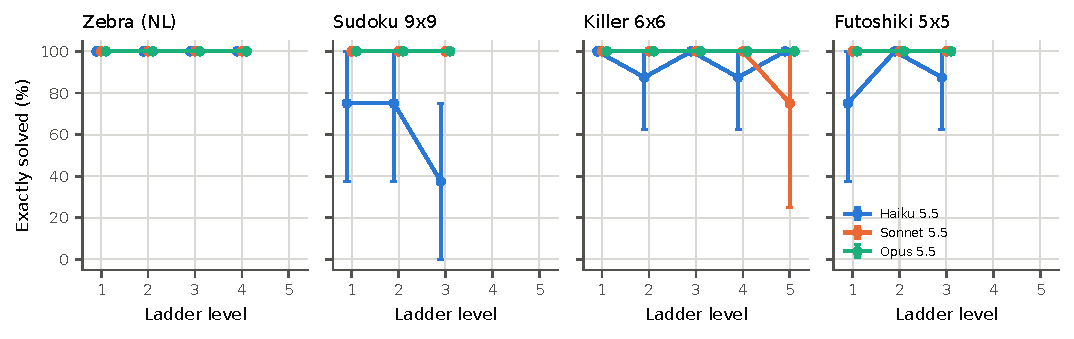
\includegraphics[width=\textwidth]{../figures/fig5_ladder_accuracy.pdf}
\caption{E3. Exact-solution rate by ladder level, family and model (95\% bootstrap intervals; 8 puzzles per cell except Killer L5 with 4). Sudoku has no L4--L5 cells because none occurred among 9{,}500 generated puzzles; Futoshiki $5{\times}5$ has none above L3.}
\label{fig:acc}
\end{figure*}

\subsection{E4: evolving fair puzzles against a solver}

\paragraph{Zebra.} A pilot on $5{\times}4$ zebra puzzles and the main run on $6{\times}6$ zebra puzzles both ended without a single training-solver error. Over \EFourZebraGens evaluated generations the $6{\times}6$ run produced \EFourZebraIndiv fair individuals (\EFourZebraLB at L2, \EFourZebraLC at L3) from \EFourZebraAccepted accepted of \EFourZebraProposals proposed edits, and Haiku solved every one of \EFourZebraEvals evaluations exactly; the pilot (\EFourPilotIndiv individuals, \EFourPilotEvals evaluations) was the same. With no error, fitness is zero everywhere and selection has nothing to act on (Figure~\ref{fig:evo}a). Fresh calls of all three models also solved every initial and final individual (Figure~\ref{fig:evo}b). Fair zebra puzzles of this size are therefore not hard for Haiku, and we stopped the zebra runs.

\paragraph{Sudoku.} PENDING


\begin{figure*}[t]
\centering
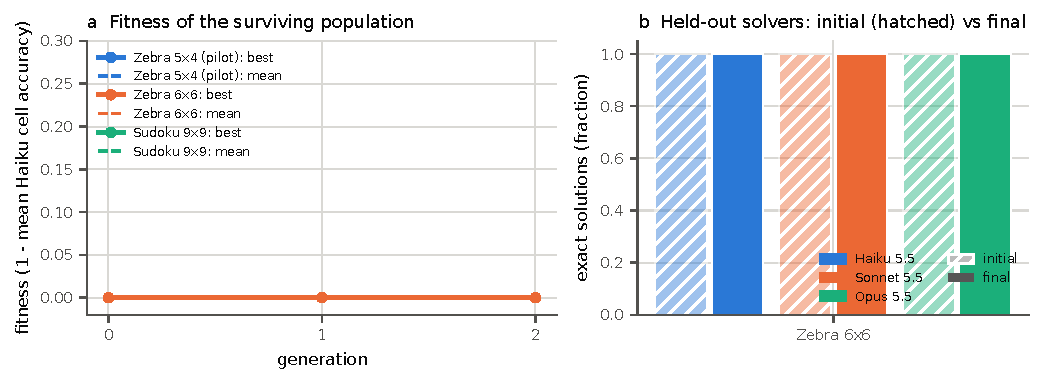
\includegraphics[width=0.85\textwidth]{../figures/fig6_evolution.pdf}
\caption{E4. (a) Best and mean fitness of the surviving population per generation (fitness = 1 $-$ mean Haiku cell accuracy over all evaluations of an individual). (b) Exact-solution rate of fresh solver calls on the initial (hatched) and final populations.}
\label{fig:evo}
\end{figure*}

\subsection{E5: genres invented by an LLM}

All \EFiveGenres genres that Sonnet wrote compiled in the sandbox, and the pipeline built and certified 12 minimal unique instances of each (Table~\ref{tab:e5}). Most genres are Latin squares with a new clue type: parity and sums of neighbours, sums of mirrored cells, cells a knight's move apart that must differ, or bans on neighbouring digits two apart. Their certified instances are mostly L3. The genre we find most interesting is \emph{Median Line Latin} (Figure~\ref{fig:gallery}e): a $5{\times}5$ Latin square whose clues either give the sum of two or three neighbouring cells or state that the middle of three consecutive cells has a value strictly between the other two. Eight of its 12 instances need two-level lookahead (L4) with about 7 clues, the deepest of all genres. The ``median'' clue is weak on its own (it rules out only the two extreme values of the middle cell) but combines with the Latin rules into long chains, which is what the ladder detects. All three models nevertheless solved all four L4 instances of this genre that we gave them (\EFiveSolveExact of \EFiveSolveN attempts).

\begin{table}[t]
\centering
\caption{E5. Genres invented by Sonnet: certified instances and their ladder levels.}
\label{tab:e5}
\small
\setlength{\tabcolsep}{3pt}
\begin{tabular}{lcrrrrrr}
\toprule
Genre & certified & L1 & L2 & L3 & L4 & L5 & clues \\
\midrule
\rows{e5_rows}
\bottomrule
\end{tabular}
\end{table}

\begin{figure*}[t]
\centering
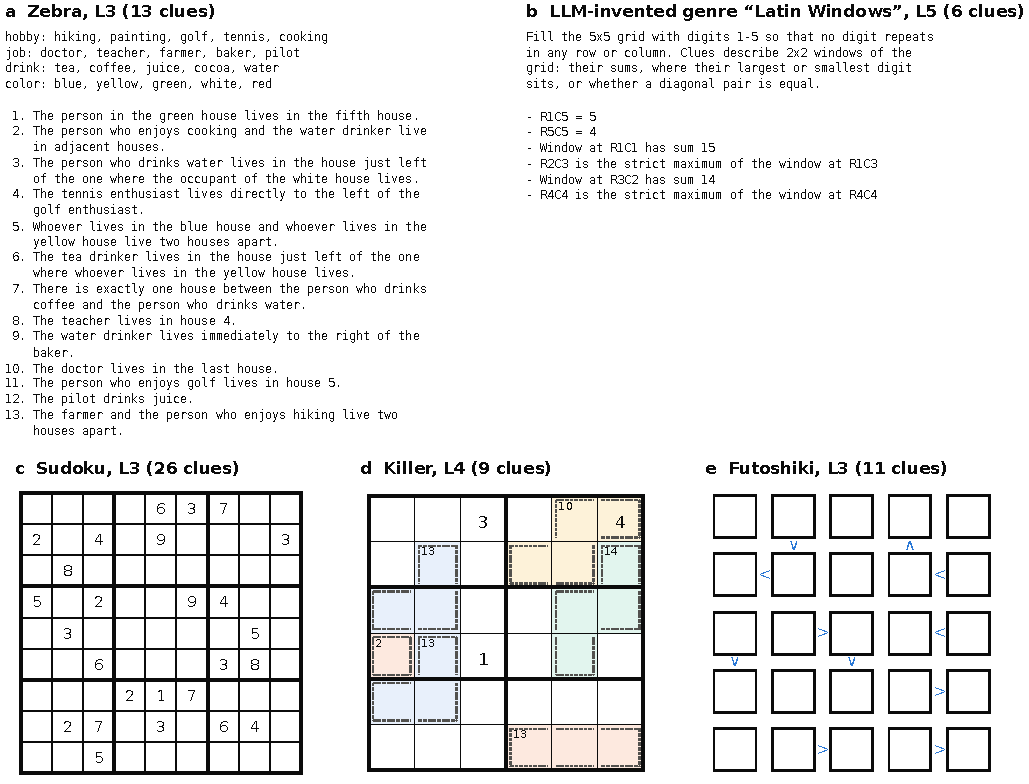
\includegraphics[width=0.92\textwidth]{../figures/fig7_gallery.pdf}
\caption{Gallery of certified puzzles from the benchmark: (a) zebra, (b) Sudoku, (c) Killer (cages with sums), (d) Futoshiki, (e) the LLM-invented genre Median Line Latin. Levels are ladder levels; every puzzle is minimal and unique.}
\label{fig:gallery}
\end{figure*}
